% Options for packages loaded elsewhere
\PassOptionsToPackage{unicode}{hyperref}
\PassOptionsToPackage{hyphens}{url}
\PassOptionsToPackage{dvipsnames,svgnames,x11names}{xcolor}
%
\documentclass[
  letterpaper,
  DIV=11,
  numbers=noendperiod]{scrartcl}

\usepackage{amsmath,amssymb}
\usepackage{iftex}
\ifPDFTeX
  \usepackage[T1]{fontenc}
  \usepackage[utf8]{inputenc}
  \usepackage{textcomp} % provide euro and other symbols
\else % if luatex or xetex
  \usepackage{unicode-math}
  \defaultfontfeatures{Scale=MatchLowercase}
  \defaultfontfeatures[\rmfamily]{Ligatures=TeX,Scale=1}
\fi
\usepackage{lmodern}
\ifPDFTeX\else  
    % xetex/luatex font selection
\fi
% Use upquote if available, for straight quotes in verbatim environments
\IfFileExists{upquote.sty}{\usepackage{upquote}}{}
\IfFileExists{microtype.sty}{% use microtype if available
  \usepackage[]{microtype}
  \UseMicrotypeSet[protrusion]{basicmath} % disable protrusion for tt fonts
}{}
\makeatletter
\@ifundefined{KOMAClassName}{% if non-KOMA class
  \IfFileExists{parskip.sty}{%
    \usepackage{parskip}
  }{% else
    \setlength{\parindent}{0pt}
    \setlength{\parskip}{6pt plus 2pt minus 1pt}}
}{% if KOMA class
  \KOMAoptions{parskip=half}}
\makeatother
\usepackage{xcolor}
\setlength{\emergencystretch}{3em} % prevent overfull lines
\setcounter{secnumdepth}{-\maxdimen} % remove section numbering
% Make \paragraph and \subparagraph free-standing
\ifx\paragraph\undefined\else
  \let\oldparagraph\paragraph
  \renewcommand{\paragraph}[1]{\oldparagraph{#1}\mbox{}}
\fi
\ifx\subparagraph\undefined\else
  \let\oldsubparagraph\subparagraph
  \renewcommand{\subparagraph}[1]{\oldsubparagraph{#1}\mbox{}}
\fi

\usepackage{color}
\usepackage{fancyvrb}
\newcommand{\VerbBar}{|}
\newcommand{\VERB}{\Verb[commandchars=\\\{\}]}
\DefineVerbatimEnvironment{Highlighting}{Verbatim}{commandchars=\\\{\}}
% Add ',fontsize=\small' for more characters per line
\usepackage{framed}
\definecolor{shadecolor}{RGB}{241,243,245}
\newenvironment{Shaded}{\begin{snugshade}}{\end{snugshade}}
\newcommand{\AlertTok}[1]{\textcolor[rgb]{0.68,0.00,0.00}{#1}}
\newcommand{\AnnotationTok}[1]{\textcolor[rgb]{0.37,0.37,0.37}{#1}}
\newcommand{\AttributeTok}[1]{\textcolor[rgb]{0.40,0.45,0.13}{#1}}
\newcommand{\BaseNTok}[1]{\textcolor[rgb]{0.68,0.00,0.00}{#1}}
\newcommand{\BuiltInTok}[1]{\textcolor[rgb]{0.00,0.23,0.31}{#1}}
\newcommand{\CharTok}[1]{\textcolor[rgb]{0.13,0.47,0.30}{#1}}
\newcommand{\CommentTok}[1]{\textcolor[rgb]{0.37,0.37,0.37}{#1}}
\newcommand{\CommentVarTok}[1]{\textcolor[rgb]{0.37,0.37,0.37}{\textit{#1}}}
\newcommand{\ConstantTok}[1]{\textcolor[rgb]{0.56,0.35,0.01}{#1}}
\newcommand{\ControlFlowTok}[1]{\textcolor[rgb]{0.00,0.23,0.31}{#1}}
\newcommand{\DataTypeTok}[1]{\textcolor[rgb]{0.68,0.00,0.00}{#1}}
\newcommand{\DecValTok}[1]{\textcolor[rgb]{0.68,0.00,0.00}{#1}}
\newcommand{\DocumentationTok}[1]{\textcolor[rgb]{0.37,0.37,0.37}{\textit{#1}}}
\newcommand{\ErrorTok}[1]{\textcolor[rgb]{0.68,0.00,0.00}{#1}}
\newcommand{\ExtensionTok}[1]{\textcolor[rgb]{0.00,0.23,0.31}{#1}}
\newcommand{\FloatTok}[1]{\textcolor[rgb]{0.68,0.00,0.00}{#1}}
\newcommand{\FunctionTok}[1]{\textcolor[rgb]{0.28,0.35,0.67}{#1}}
\newcommand{\ImportTok}[1]{\textcolor[rgb]{0.00,0.46,0.62}{#1}}
\newcommand{\InformationTok}[1]{\textcolor[rgb]{0.37,0.37,0.37}{#1}}
\newcommand{\KeywordTok}[1]{\textcolor[rgb]{0.00,0.23,0.31}{#1}}
\newcommand{\NormalTok}[1]{\textcolor[rgb]{0.00,0.23,0.31}{#1}}
\newcommand{\OperatorTok}[1]{\textcolor[rgb]{0.37,0.37,0.37}{#1}}
\newcommand{\OtherTok}[1]{\textcolor[rgb]{0.00,0.23,0.31}{#1}}
\newcommand{\PreprocessorTok}[1]{\textcolor[rgb]{0.68,0.00,0.00}{#1}}
\newcommand{\RegionMarkerTok}[1]{\textcolor[rgb]{0.00,0.23,0.31}{#1}}
\newcommand{\SpecialCharTok}[1]{\textcolor[rgb]{0.37,0.37,0.37}{#1}}
\newcommand{\SpecialStringTok}[1]{\textcolor[rgb]{0.13,0.47,0.30}{#1}}
\newcommand{\StringTok}[1]{\textcolor[rgb]{0.13,0.47,0.30}{#1}}
\newcommand{\VariableTok}[1]{\textcolor[rgb]{0.07,0.07,0.07}{#1}}
\newcommand{\VerbatimStringTok}[1]{\textcolor[rgb]{0.13,0.47,0.30}{#1}}
\newcommand{\WarningTok}[1]{\textcolor[rgb]{0.37,0.37,0.37}{\textit{#1}}}

\providecommand{\tightlist}{%
  \setlength{\itemsep}{0pt}\setlength{\parskip}{0pt}}\usepackage{longtable,booktabs,array}
\usepackage{calc} % for calculating minipage widths
% Correct order of tables after \paragraph or \subparagraph
\usepackage{etoolbox}
\makeatletter
\patchcmd\longtable{\par}{\if@noskipsec\mbox{}\fi\par}{}{}
\makeatother
% Allow footnotes in longtable head/foot
\IfFileExists{footnotehyper.sty}{\usepackage{footnotehyper}}{\usepackage{footnote}}
\makesavenoteenv{longtable}
\usepackage{graphicx}
\makeatletter
\def\maxwidth{\ifdim\Gin@nat@width>\linewidth\linewidth\else\Gin@nat@width\fi}
\def\maxheight{\ifdim\Gin@nat@height>\textheight\textheight\else\Gin@nat@height\fi}
\makeatother
% Scale images if necessary, so that they will not overflow the page
% margins by default, and it is still possible to overwrite the defaults
% using explicit options in \includegraphics[width, height, ...]{}
\setkeys{Gin}{width=\maxwidth,height=\maxheight,keepaspectratio}
% Set default figure placement to htbp
\makeatletter
\def\fps@figure{htbp}
\makeatother

\KOMAoption{captions}{tableheading}
\makeatletter
\makeatother
\makeatletter
\makeatother
\makeatletter
\@ifpackageloaded{caption}{}{\usepackage{caption}}
\AtBeginDocument{%
\ifdefined\contentsname
  \renewcommand*\contentsname{Table of contents}
\else
  \newcommand\contentsname{Table of contents}
\fi
\ifdefined\listfigurename
  \renewcommand*\listfigurename{List of Figures}
\else
  \newcommand\listfigurename{List of Figures}
\fi
\ifdefined\listtablename
  \renewcommand*\listtablename{List of Tables}
\else
  \newcommand\listtablename{List of Tables}
\fi
\ifdefined\figurename
  \renewcommand*\figurename{Figure}
\else
  \newcommand\figurename{Figure}
\fi
\ifdefined\tablename
  \renewcommand*\tablename{Table}
\else
  \newcommand\tablename{Table}
\fi
}
\@ifpackageloaded{float}{}{\usepackage{float}}
\floatstyle{ruled}
\@ifundefined{c@chapter}{\newfloat{codelisting}{h}{lop}}{\newfloat{codelisting}{h}{lop}[chapter]}
\floatname{codelisting}{Listing}
\newcommand*\listoflistings{\listof{codelisting}{List of Listings}}
\makeatother
\makeatletter
\@ifpackageloaded{caption}{}{\usepackage{caption}}
\@ifpackageloaded{subcaption}{}{\usepackage{subcaption}}
\makeatother
\makeatletter
\@ifpackageloaded{tcolorbox}{}{\usepackage[skins,breakable]{tcolorbox}}
\makeatother
\makeatletter
\@ifundefined{shadecolor}{\definecolor{shadecolor}{rgb}{.97, .97, .97}}
\makeatother
\makeatletter
\makeatother
\makeatletter
\makeatother
\ifLuaTeX
  \usepackage{selnolig}  % disable illegal ligatures
\fi
\IfFileExists{bookmark.sty}{\usepackage{bookmark}}{\usepackage{hyperref}}
\IfFileExists{xurl.sty}{\usepackage{xurl}}{} % add URL line breaks if available
\urlstyle{same} % disable monospaced font for URLs
\hypersetup{
  pdftitle={Beispiel: Kragarm mit 2 Punktmassen},
  colorlinks=true,
  linkcolor={blue},
  filecolor={Maroon},
  citecolor={Blue},
  urlcolor={Blue},
  pdfcreator={LaTeX via pandoc}}

\title{Beispiel: Kragarm mit 2 Punktmassen}
\author{}
\date{}

\begin{document}
\maketitle
\ifdefined\Shaded\renewenvironment{Shaded}{\begin{tcolorbox}[enhanced, boxrule=0pt, interior hidden, sharp corners, frame hidden, borderline west={3pt}{0pt}{shadecolor}, breakable]}{\end{tcolorbox}}\fi

\begin{Shaded}
\begin{Highlighting}[]
\ImportTok{from}\NormalTok{ sympycalcs.helpers }\ImportTok{import}\NormalTok{ Equation }\ImportTok{as}\NormalTok{ Eqn}
\ImportTok{from}\NormalTok{ sympycalcs }\ImportTok{import}\NormalTok{ render, convert}
\ImportTok{import}\NormalTok{ sympy }\ImportTok{as}\NormalTok{ sp }

\ImportTok{import}\NormalTok{ sympy.physics.units }\ImportTok{as}\NormalTok{ unit}
\ImportTok{from}\NormalTok{ sympy.abc }\ImportTok{import} \OperatorTok{*}
\NormalTok{sp.init\_printing(use\_latex}\OperatorTok{=}\StringTok{\textquotesingle{}mathjax\textquotesingle{}}\NormalTok{, latex\_mode}\OperatorTok{=}\StringTok{\textquotesingle{}equation\textquotesingle{}}\NormalTok{)}
\end{Highlighting}
\end{Shaded}

\newpage{}

\hypertarget{aufgabenstellung}{%
\subsection{Aufgabenstellung}\label{aufgabenstellung}}

Das in Figure~\ref{fig-kragarm_2_punkte} dargestellte System stellt
einen Kragarm mit verteilter Masse und 2 Punktmassen dar. Eine mögliche
Formfunktion ist rechts daneben gezeigt.

\begin{figure}

{\centering 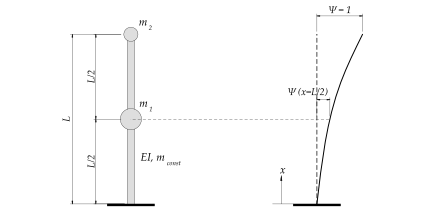
\includegraphics{example_rayleigh_files/mediabag/bilder/aufgabe_rayleigh_2_massen.pdf}

}

\caption{\label{fig-kragarm_2_punkte}Kragarm mit verteilter Masse und
zwei Punktmassen}

\end{figure}

Gesucht:

\begin{itemize}
\tightlist
\item
  Grundfrequenz (1. Eigenfrequenz \(\omega_n\)) des Systems, berechnet
  mit dem Rayleigh-Quotienten.
\end{itemize}

Gegeben:

\begin{itemize}
\tightlist
\item
  Randbedingungen für den Spezialfall:
  \(m_{const} = 0 \text{ und } m_1 = m_2 = m\)
\item
  Formfunktion: \[ \Psi(x) = 1 - \cos(\frac{\pi x}{2L})\]
\end{itemize}

\begin{Shaded}
\begin{Highlighting}[]
\NormalTok{L }\OperatorTok{=}\NormalTok{ sp.symbols(}\StringTok{\textquotesingle{}L\textquotesingle{}}\NormalTok{, positive}\OperatorTok{=}\VariableTok{True}\NormalTok{)}
\NormalTok{m\_1, m\_2, m\_star, k\_star, omega\_1 }\OperatorTok{=}\NormalTok{ sp.symbols(}\StringTok{\textquotesingle{}m\_1, m\_2, m\_star, k\_star omega\_1\textquotesingle{}}\NormalTok{)}

\NormalTok{Psi\_x }\OperatorTok{=}\NormalTok{ sp.Function(}\StringTok{\textquotesingle{}Psi\textquotesingle{}}\NormalTok{)(x)}
\NormalTok{f }\OperatorTok{=}\NormalTok{ sp.Function(}\StringTok{\textquotesingle{}f\textquotesingle{}}\NormalTok{)(x,t)}
\end{Highlighting}
\end{Shaded}

\begin{Shaded}
\begin{Highlighting}[]
\NormalTok{params}\OperatorTok{=}\NormalTok{\{}
\NormalTok{    m:}\DecValTok{0}\NormalTok{,}
\NormalTok{    m\_1:m,}
\NormalTok{    m\_2:m}
\NormalTok{\}}
\end{Highlighting}
\end{Shaded}

\newpage{}

\hypertarget{musterluxf6sung}{%
\subsection{Musterlösung}\label{musterluxf6sung}}

\hypertarget{formfunktion}{%
\subsubsection{Formfunktion}\label{formfunktion}}

\begin{Shaded}
\begin{Highlighting}[]
\NormalTok{eq\_Psi\_x }\OperatorTok{=}\NormalTok{ Eqn(Psi\_x, }\DecValTok{1} \OperatorTok{{-}}\NormalTok{ sp.cos(sp.pi}\OperatorTok{*}\NormalTok{x}\OperatorTok{/}\NormalTok{(}\DecValTok{2}\OperatorTok{*}\NormalTok{L)))}
\NormalTok{eq\_Psi\_x}
\end{Highlighting}
\end{Shaded}

\begin{equation}\Psi{\left(x \right)} = 1 - \cos{\left(\frac{\pi x}{2 L} \right)}\end{equation}

\hypertarget{allgemeine-bewegungsgleichung}{%
\subsubsection{Allgemeine
Bewegungsgleichung}\label{allgemeine-bewegungsgleichung}}

Mithilfe der in der Vorlesung hergeleiteten Bewegungsgleichung kann
anhand der Formfunktion \(\Psi\) die erste Eigenkreisfrequenz ermittelt
werden. Der Rayleigh-Quotient ist eine Energiebetrachtung. Er setzt die
potentielle, maximale Energie \(E_{pot,max}\) zur kinetischen, maximalen
Energie \(E_{kin,max}\) ins Verhältnis. Daraus lässt sich die
Kreisfrequenz \(\omega_n\) herauslösen.

\begin{Shaded}
\begin{Highlighting}[]
\NormalTok{eq\_m\_star }\OperatorTok{=}\NormalTok{ Eqn(m\_star,sp.Integral(m}\OperatorTok{*}\NormalTok{Psi\_x}\OperatorTok{**}\DecValTok{2}\NormalTok{,(x, }\DecValTok{0}\NormalTok{,L))}\OperatorTok{+}\NormalTok{m\_1 }\OperatorTok{*}\NormalTok{ Psi\_x.subs(x,L)}\OperatorTok{**}\DecValTok{2} \OperatorTok{+}\NormalTok{ m\_2 }\OperatorTok{*}\NormalTok{Psi\_x.subs(x,L}\OperatorTok{/}\DecValTok{2}\NormalTok{)}\OperatorTok{**}\DecValTok{2}\NormalTok{)}
\NormalTok{eq\_k\_star }\OperatorTok{=}\NormalTok{ Eqn(k\_star,sp.Integral(E}\OperatorTok{*}\NormalTok{I}\OperatorTok{*}\NormalTok{sp.Derivative(Psi\_x,x,}\DecValTok{2}\NormalTok{)}\OperatorTok{**}\DecValTok{2}\NormalTok{, (x,}\DecValTok{0}\NormalTok{,L)))}
\NormalTok{display(eq\_m\_star, eq\_k\_star)}
\end{Highlighting}
\end{Shaded}

\begin{equation}m_{star} = m_{1} \Psi^{2}{\left(L \right)} + m_{2} \Psi^{2}{\left(\frac{L}{2} \right)} + \int\limits_{0}^{L} m \Psi^{2}{\left(x \right)}\, dx\end{equation}

\begin{equation}k_{star} = \int\limits_{0}^{L} E I \left(\frac{d^{2}}{d x^{2}} \Psi{\left(x \right)}\right)^{2}\, dx\end{equation}

\begin{Shaded}
\begin{Highlighting}[]
\NormalTok{eq\_bewegung\_allg }\OperatorTok{=}\NormalTok{ Eqn(f, sp.Derivative(u,x,}\DecValTok{2}\NormalTok{)}\OperatorTok{*}\NormalTok{m\_star}\OperatorTok{+}\NormalTok{u}\OperatorTok{*}\NormalTok{k\_star)}
\NormalTok{eq\_bewegung\_allg}
\end{Highlighting}
\end{Shaded}

\begin{equation}f{\left(x,t \right)} = k_{star} u + m_{star} \frac{d^{2}}{d x^{2}} u\end{equation}

\begin{Shaded}
\begin{Highlighting}[]
\NormalTok{eq\_bewegung\_allg.subs(eq\_m\_star, eq\_k\_star)}
\end{Highlighting}
\end{Shaded}

\begin{equation}f{\left(x,t \right)} = u \int\limits_{0}^{L} E I \left(\frac{d^{2}}{d x^{2}} \Psi{\left(x \right)}\right)^{2}\, dx + \left(m_{1} \Psi^{2}{\left(L \right)} + m_{2} \Psi^{2}{\left(\frac{L}{2} \right)} + \int\limits_{0}^{L} m \Psi^{2}{\left(x \right)}\, dx\right) \frac{d^{2}}{d x^{2}} u\end{equation}

Substituiert mit Massen- und Steifigkeitsvariable:

\hypertarget{eigenkreisfrequenz}{%
\subsubsection{Eigenkreisfrequenz}\label{eigenkreisfrequenz}}

Aus der Bewegungsgleichung kann die Eigenkreisfrequenz ermittelt werden:

\begin{Shaded}
\begin{Highlighting}[]
\NormalTok{eq\_eigenkreisfreq }\OperatorTok{=}\NormalTok{ Eqn(omega\_1, sp.sqrt(k\_star}\OperatorTok{/}\NormalTok{ m\_star))}
\NormalTok{eq\_eigenkreisfreq}
\end{Highlighting}
\end{Shaded}

\begin{equation}\omega_{1} = \sqrt{\frac{k_{star}}{m_{star}}}\end{equation}

\hypertarget{bestimmung-der-masse}{%
\paragraph{Bestimmung der Masse}\label{bestimmung-der-masse}}

Die Masse kann mittels der Lösung des Integrals bestimmt werden. Dabei
sind die Punktmassen mittels der entsprechenden Deformation an den
Stellen \(L\) und \(\frac{L}{2}\) zu berücksichtigen, sowie die
verteilte Masse über die gesamte Länge.

\begin{Shaded}
\begin{Highlighting}[]
\NormalTok{eq\_Psi\_x.subs(x,L)}
\end{Highlighting}
\end{Shaded}

\begin{equation}\Psi{\left(L \right)} = 1\end{equation}

\begin{Shaded}
\begin{Highlighting}[]
\NormalTok{eq\_Psi\_x.subs(x,L}\OperatorTok{/}\DecValTok{2}\NormalTok{)}
\end{Highlighting}
\end{Shaded}

\begin{equation}\Psi{\left(\frac{L}{2} \right)} = 1 - \frac{\sqrt{2}}{2}\end{equation}

\begin{Shaded}
\begin{Highlighting}[]
\NormalTok{eq\_Psi\_x}\OperatorTok{**}\DecValTok{2}
\end{Highlighting}
\end{Shaded}

\begin{equation}\Psi^{2}{\left(x \right)} = \left(1 - \cos{\left(\frac{\pi x}{2 L} \right)}\right)^{2}\end{equation}

\begin{Shaded}
\begin{Highlighting}[]
\NormalTok{eq\_m\_star.subs(eq\_Psi\_x, eq\_Psi\_x.subs(x,L), eq\_Psi\_x.subs(x,L}\OperatorTok{/}\DecValTok{2}\NormalTok{))}
\end{Highlighting}
\end{Shaded}

\begin{equation}m_{star} = m_{1} + m_{2} \left(1 - \frac{\sqrt{2}}{2}\right)^{2} + \int\limits_{0}^{L} m \left(1 - \cos{\left(\frac{\pi x}{2 L} \right)}\right)^{2}\, dx\end{equation}

\begin{Shaded}
\begin{Highlighting}[]
\NormalTok{eq\_m\_star.subs(eq\_Psi\_x, eq\_Psi\_x.subs(x,L), eq\_Psi\_x.subs(x,L}\OperatorTok{/}\DecValTok{2}\NormalTok{)).doit()}
\end{Highlighting}
\end{Shaded}

\begin{equation}m_{star} = m \left(- \frac{4 L}{\pi} + \frac{3 L}{2}\right) + m_{1} + m_{2} \left(1 - \frac{\sqrt{2}}{2}\right)^{2}\end{equation}

\hypertarget{bestimmung-der-steifigkeit}{%
\paragraph{Bestimmung der
Steifigkeit}\label{bestimmung-der-steifigkeit}}

Die Steifigkeit in kann mittels der Lösung des Integrals in bestimmt
werden. Zur Ermittlung der Steifigkeit \(k^\star\) muss zuerst der
Ansatz zweimal nach \(x\) abgeleitet werden.

\begin{Shaded}
\begin{Highlighting}[]
\NormalTok{display(eq\_Psi\_x,sp.diff(eq\_Psi\_x,x,}\DecValTok{1}\NormalTok{),sp.diff(eq\_Psi\_x,x,}\DecValTok{2}\NormalTok{))}
\end{Highlighting}
\end{Shaded}

\begin{equation}\Psi{\left(x \right)} = 1 - \cos{\left(\frac{\pi x}{2 L} \right)}\end{equation}

\begin{equation}\frac{d}{d x} \Psi{\left(x \right)} = \frac{\pi \sin{\left(\frac{\pi x}{2 L} \right)}}{2 L}\end{equation}

\begin{equation}\frac{d^{2}}{d x^{2}} \Psi{\left(x \right)} = \frac{\pi^{2} \cos{\left(\frac{\pi x}{2 L} \right)}}{4 L^{2}}\end{equation}

Danach bedingt es lediglich das einsetzen:

\begin{Shaded}
\begin{Highlighting}[]
\NormalTok{display(eq\_k\_star.subs(eq\_Psi\_x),}
\NormalTok{       eq\_k\_star.subs(eq\_Psi\_x).doit())}
\end{Highlighting}
\end{Shaded}

\begin{equation}k_{star} = \int\limits_{0}^{L} E I \left(\frac{\partial^{2}}{\partial x^{2}} \left(1 - \cos{\left(\frac{\pi x}{2 L} \right)}\right)\right)^{2}\, dx\end{equation}

\begin{equation}k_{star} = \frac{\pi^{4} E I}{32 L^{3}}\end{equation}

\hypertarget{grundfrequenz}{%
\paragraph{Grundfrequenz}\label{grundfrequenz}}

Letztlich kann die Grundfrequenz bestimmt werden:

\begin{Shaded}
\begin{Highlighting}[]
\NormalTok{omega\_1\_sub }\OperatorTok{=}\NormalTok{ eq\_eigenkreisfreq.subs(eq\_k\_star, eq\_m\_star).subs(eq\_Psi\_x, eq\_Psi\_x.subs(x,L), eq\_Psi\_x.subs(x,L}\OperatorTok{/}\DecValTok{2}\NormalTok{)).simplify()}

\NormalTok{omega\_1\_sub}
\end{Highlighting}
\end{Shaded}

\begin{equation}\omega_{1} = \frac{\sqrt{2} \pi^{2} \sqrt{\frac{E I}{4 m \left(- \frac{4 L}{\pi} + \frac{3 L}{2}\right) + 4 m_{1} + m_{2} \left(-2 + \sqrt{2}\right)^{2}}}}{4 L^{\frac{3}{2}}}\end{equation}

\hypertarget{auswertung-des-spezialfalls}{%
\paragraph{Auswertung des
Spezialfalls}\label{auswertung-des-spezialfalls}}

Mit Hilfe der Randbedingungen für den Spezialfall aus der
Aufgabenstellung resultiert die Grundfrequenz zu:

\begin{Shaded}
\begin{Highlighting}[]
\NormalTok{omega\_1\_sub.subs(params).simplify().evalf(}\DecValTok{3}\NormalTok{)}
\end{Highlighting}
\end{Shaded}

\begin{equation}\omega_{1} = \frac{1.67 \left(\frac{E I}{m}\right)^{0.5}}{L^{1.5}}\end{equation}



\end{document}
